\documentclass{article}

\usepackage{fullpage,verbatim,amsmath,graphicx,listings,color}

\newcommand{\HRule}{\rule{\linewidth}{0.5mm}}
\begin{document}

\lstset{
language=Python, 
basicstyle=\scriptsize,
backgroundcolor=\color{white},
showspaces=false,
showstringspaces=false,
showtabs=false,
frame=shadowbox,
tabsize=4,
captionpos=b,
title=\lstname,
breaklines=true,
breakatwhitespace=true}

\begin{titlepage}
 
\begin{center}
 
\textsc{\LARGE Homework 5}\\[1.5cm] 

\textsc{\Large Computational Math}\\[0.5cm]
 
 
\HRule \\[2cm]
 
% Author and supervisor
\begin{minipage}{0.4\textwidth}
\begin{flushleft} \large
\emph{Author:}\\
Mikola Lysenko
\end{flushleft}
\end{minipage}
 
\vfill
 
% Bottom of the page
{\large \today}
 
\end{center}
 
\end{titlepage}


\paragraph{1}

\subparagraph{a}
For the test functions, choose $u,v$ from the space of continuous functions supported on $\Omega$; ie $\text{supp } u \subseteq \Omega$.  Now for any solution $u$ with test function $v$ we must have:
\[ \int \limits_{\Omega} - u_{xx}(x,y) v(x,y) - u_{yy}(x,y) v(x,y) d \Omega = \int \limits_{\Omega} f(x,y) v(x,y) d \Omega \]
Starting on the left hand side, we work term by term:
\begin{eqnarray*}
\int \limits_{-1}^{1} \int \limits_{-1}^{1} -u_{xx}(x,y) v(x,y) dx dy & = &
\int \limits_{-1}^{1} \left( -u_x(x,y) v(x,y) |_{-1}^{1} + \int \limits_{-1}^{1} u_{x}(x,y) v_{x}(x,y) dx \right) dy \\
& = & \int \limits_{\Omega} u_{x}(x,y) v_{x}(x,y) d \Omega \\
& = & p_1(u, v)
\end{eqnarray*}
By symmetry:
\[ p_2(u,v) = \int \limits_{\Omega} u_{yy} v d \Omega = \int \limits_{\Omega} u_{y}(x,y) v_{y}(x,y) d \Omega \]
For the right hand side, we just get:
\[ b(v) = \int \limits_{\Omega} f(x,y) v(x,y) d \Omega \]
And so the weak form of the variational problem is:
\[ p_1(u,v) + p_2(u,v) = b(v) \]

\subparagraph{b}

Let $(x_1, y_1), (x_2, y_2), (x_3, y_3), (x_4, y_4)$ be the nodes of the element, oriented clockwise.  We now solve for $\alpha_1, \alpha_2, \alpha_3, \alpha_4$ for the node $(x_1, y_1)$.  Plugging in values, we get the following linear system:
\begin{eqnarray*}
\alpha_1 + \alpha_2 x_1 + \alpha_3 y_1 + \alpha_4 x_1 y_1 & = & 1 \\
\alpha_1 + \alpha_2 x_2 + \alpha_3 y_2 + \alpha_4 x_1 y_2 & = & 0 \\
\alpha_1 + \alpha_2 x_3 + \alpha_3 y_3 + \alpha_4 x_1 y_3 & = & 0 \\
\alpha_1 + \alpha_2 x_4 + \alpha_3 y_4 + \alpha_4 x_4 y_4 & = & 0
\end{eqnarray*}
For the sake of simplicity, we rewrite the system in matrix form:
\[ M \alpha = c \]
Where $\alpha$ is the vector of coefficients. Since $c$ is a basis vector, the values for $\alpha$ at various nodes are just the corresponding rows of $M^{-1}$.  

Now to construct the matrix equations for this system, we first consider the weak form from part a on a per element basis.  Thus let $\varphi^i, \varphi^j$ be two test functions on a quad element where
\[ \varphi^i(x) = \alpha^i_1 + \alpha^i_2 x + \alpha^i_3 y + \alpha^i_4 x y \]
And:
\[ \varphi^i_{x}(x) = \alpha^i_2 + \alpha^i_4 y \]
To integrate $p_1(\varphi^i, \varphi^j)$, we split the integral into two triangles, indexed by $\Delta(1, 2, 3)$ and $\Delta(1, 3, 4)$, then integrate in barycentric coordinates.  We do this for the first triangle $\Delta(1,2,3)$ now.  Let:
\[ J = \left( \begin{array}{cc}
x_2 - x_1 & y_2 - y_1 \\
x_3 - x_1 & y_3 - y_1
\end{array} \right) \]
And define the affine transformation:
\[ \mathcal{T}(\lambda_1, \lambda_2) = J \left( \begin{array}{c}
\lambda_1 \\
\lambda_2 \\
\end{array} \right) + \left( \begin{array}{c}
x_1 \\
y_1 \\
\end{array} \right) \]
And so we get the following:
\begin{eqnarray*}
\int \limits_{\Delta(1,2,3)} \varphi^i_x(x,y) \varphi^j_x(x,y) d x d y & = & 
\frac{1}{\det J} \int \limits_{0}^{1} \int \limits_{0}^{1- \lambda_2} \varphi^i_{x}(\mathcal{T} (\lambda_1, \lambda_2)) \varphi^j_{x}(\mathcal{T}(\lambda_1, \lambda_2))) d \lambda_1 d \lambda_2  \\
& = & \frac{1}{\det J} \int \limits_{0}^{1} \int \limits_{0}^{1 - \lambda_2}
\alpha^i_2 \alpha^j_2 + (\alpha^i_4 \alpha^j_2  + \alpha^i_2 \alpha^j_4) (J_{2,1} \lambda_1 + J_{2,2} \lambda_2 + y_1) \\
& & \:\:\:\:\:\:\:\:\:\:\:\:\:\: + \:\: \alpha^i_4 \alpha^j_4 (J_{2,1} \lambda_1 + J_{2,2} \lambda_2 + y_1)^2 d \lambda_1 d \lambda_2 
\end{eqnarray*}
To simplify the expression, make the following substitutions:
\begin{eqnarray*}
Q_0 & = & \alpha^i_2 \alpha^j_2 \\
Q_1 & = & \alpha^i_2 \alpha^j_4 + \alpha^i_4 \alpha^j_2 \\
Q_2 & = & \alpha^i_4 \alpha^j_4
\end{eqnarray*}
And so we get the following quantity:
\[ = \frac{1}{2\det J} \left( 
  Q_0 + y_1 \left( Q_1 + y_1 Q_2 \right)
+ \frac{J_{2,1} + J_{2,2}}{3} \left(  
   Q_1 + \left( 2 y_1 + \frac{J_{2,1} + J_{2,2}}{2} \right) Q_2 \right)  - \frac{J_{2,1} J_{2,2} Q_2}{6} \right) \]
We shall call this quantity $T^1_1$, where the upper index denotes the triangle and the lower index denotes the $p_1$ component of the Laplacian, thus we get:
\[ A(\varphi^i, \varphi^j) = p_1(\varphi^i, \varphi^j) + p_2(\varphi^i, \varphi^j) = \sum T^1_1 + T^1_2 + T^2_1 + T^2_2 \]
And so the final matrix is just formed by summing over all such values.  Computing $f$ can be done approximately by sampling at the nodal values.

\subparagraph{c}

Here is the code I wrote to implement the described method (in Python):

\pagebreak
\lstinputlisting{prob1.py}

And here is a heatmap plot of the resulting distribution:

\begin{center}
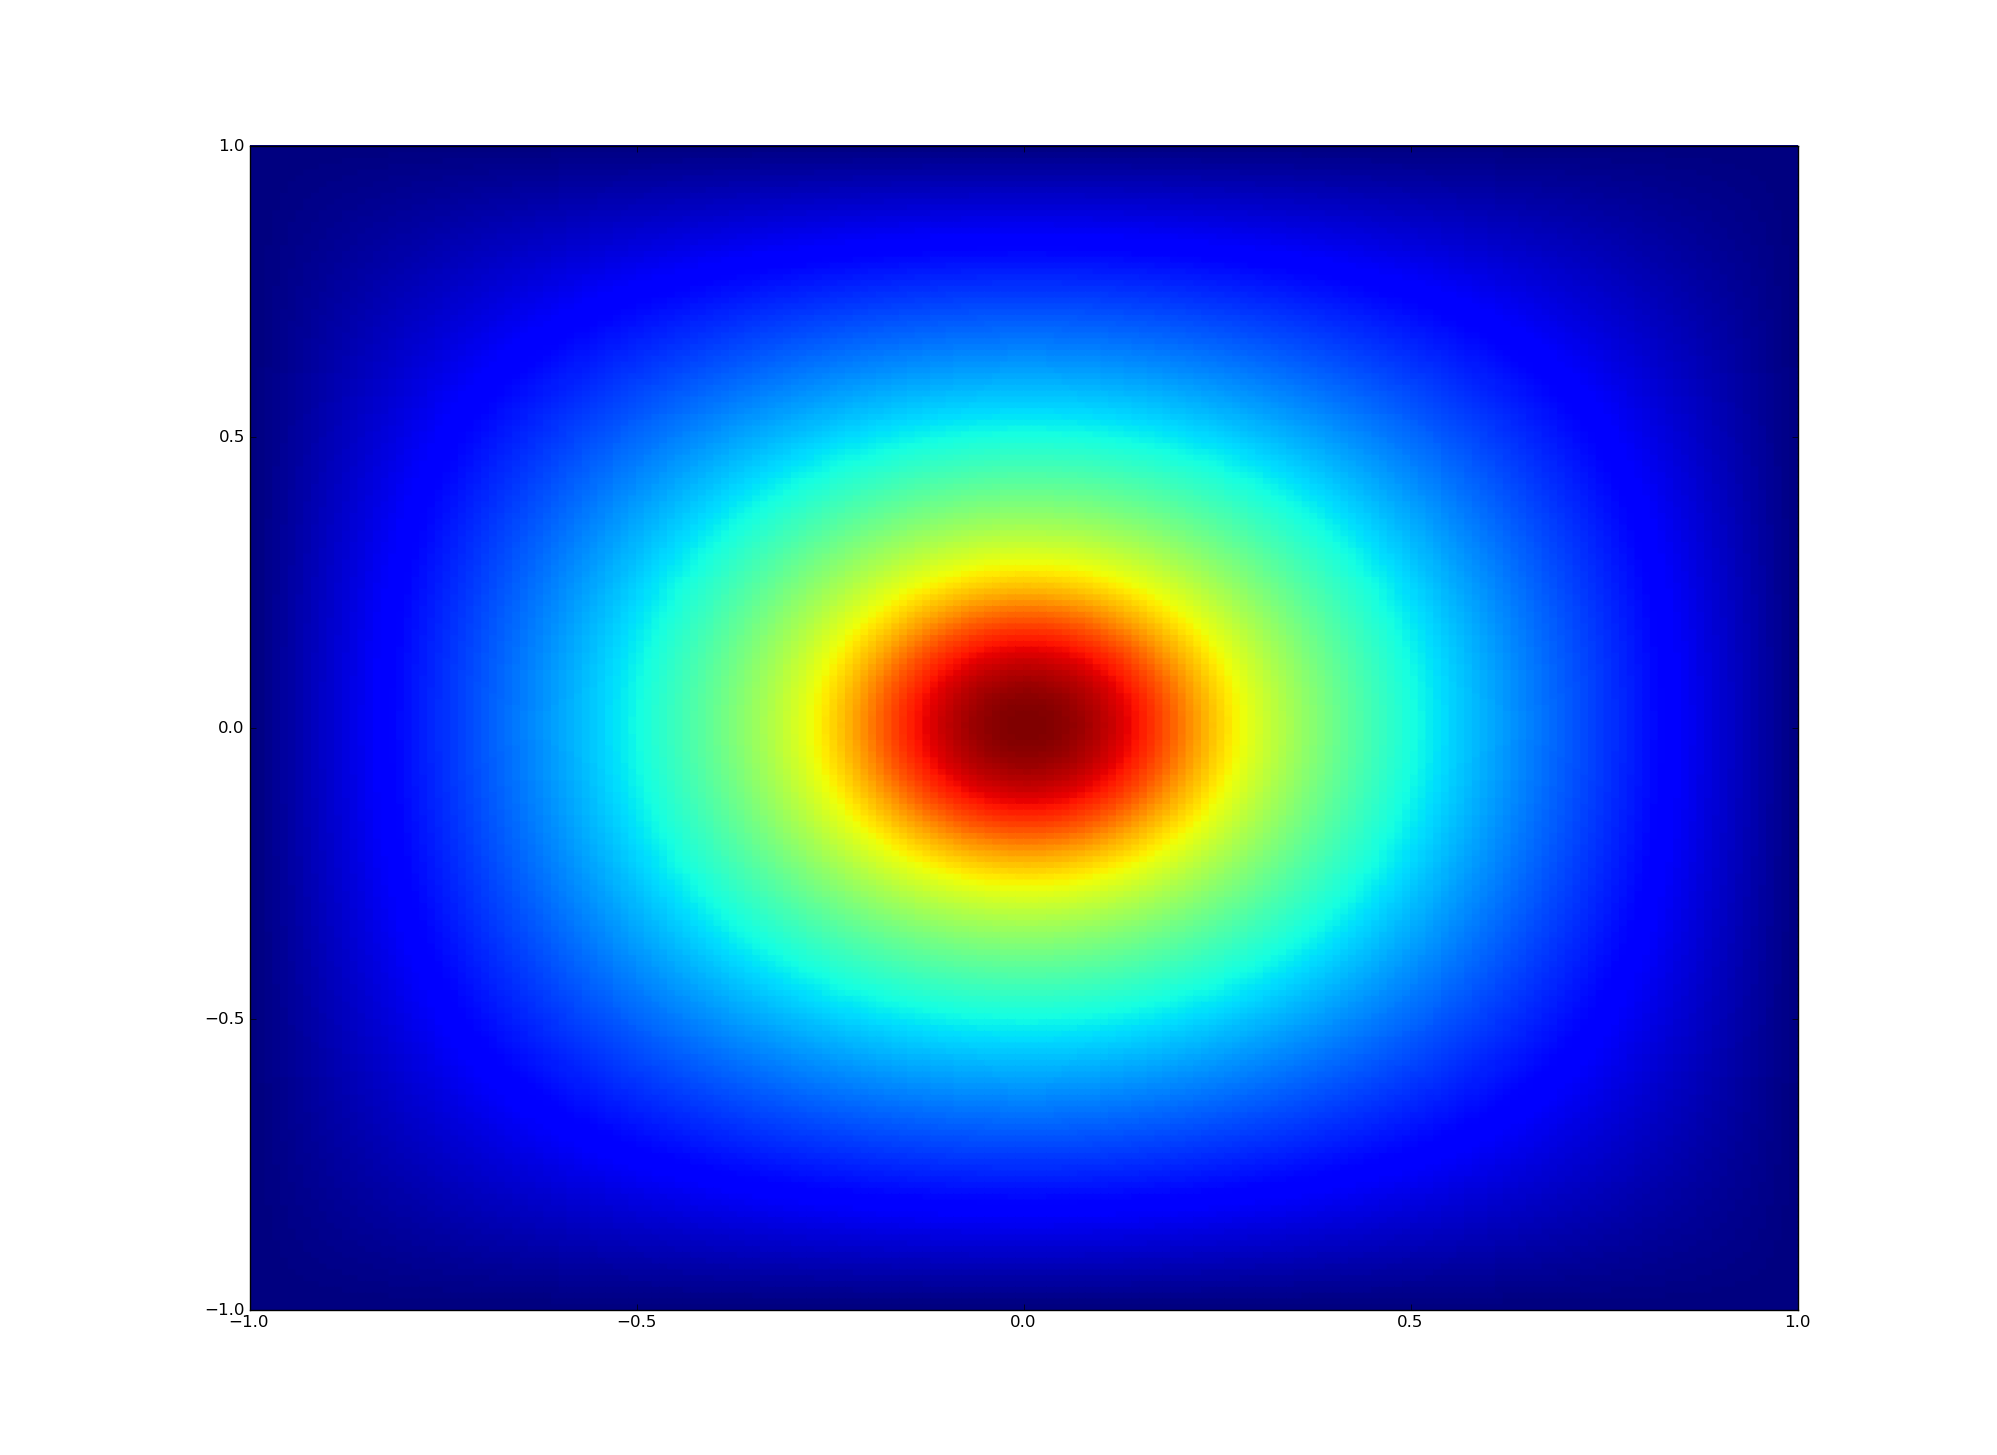
\includegraphics[width=5in]{prob1_result.png}
\end{center}

\paragraph{2}

\paragraph{3}

\paragraph{4}

\end{document}
